\documentclass{article}\usepackage[]{graphicx}\usepackage[]{color}
%% maxwidth is the original width if it is less than linewidth
%% otherwise use linewidth (to make sure the graphics do not exceed the margin)
\makeatletter
\def\maxwidth{ %
  \ifdim\Gin@nat@width>\linewidth
    \linewidth
  \else
    \Gin@nat@width
  \fi
}
\makeatother

\definecolor{fgcolor}{rgb}{0.345, 0.345, 0.345}
\newcommand{\hlnum}[1]{\textcolor[rgb]{0.686,0.059,0.569}{#1}}%
\newcommand{\hlstr}[1]{\textcolor[rgb]{0.192,0.494,0.8}{#1}}%
\newcommand{\hlcom}[1]{\textcolor[rgb]{0.678,0.584,0.686}{\textit{#1}}}%
\newcommand{\hlopt}[1]{\textcolor[rgb]{0,0,0}{#1}}%
\newcommand{\hlstd}[1]{\textcolor[rgb]{0.345,0.345,0.345}{#1}}%
\newcommand{\hlkwa}[1]{\textcolor[rgb]{0.161,0.373,0.58}{\textbf{#1}}}%
\newcommand{\hlkwb}[1]{\textcolor[rgb]{0.69,0.353,0.396}{#1}}%
\newcommand{\hlkwc}[1]{\textcolor[rgb]{0.333,0.667,0.333}{#1}}%
\newcommand{\hlkwd}[1]{\textcolor[rgb]{0.737,0.353,0.396}{\textbf{#1}}}%

\usepackage{framed}
\makeatletter
\newenvironment{kframe}{%
 \def\at@end@of@kframe{}%
 \ifinner\ifhmode%
  \def\at@end@of@kframe{\end{minipage}}%
  \begin{minipage}{\columnwidth}%
 \fi\fi%
 \def\FrameCommand##1{\hskip\@totalleftmargin \hskip-\fboxsep
 \colorbox{shadecolor}{##1}\hskip-\fboxsep
     % There is no \\@totalrightmargin, so:
     \hskip-\linewidth \hskip-\@totalleftmargin \hskip\columnwidth}%
 \MakeFramed {\advance\hsize-\width
   \@totalleftmargin\z@ \linewidth\hsize
   \@setminipage}}%
 {\par\unskip\endMakeFramed%
 \at@end@of@kframe}
\makeatother

\definecolor{shadecolor}{rgb}{.97, .97, .97}
\definecolor{messagecolor}{rgb}{0, 0, 0}
\definecolor{warningcolor}{rgb}{1, 0, 1}
\definecolor{errorcolor}{rgb}{1, 0, 0}
\newenvironment{knitrout}{}{} % an empty environment to be redefined in TeX

\usepackage{alltt}
\usepackage{Sweave}
\usepackage{float}
\usepackage{graphicx}
\usepackage{tabularx}
\usepackage[comma]{natbib}
\bibliographystyle{agsm} 
\usepackage[small]{caption}
\setkeys{Gin}{width=0.8\textwidth}
\setlength{\captionmargin}{30pt}
\setlength{\abovecaptionskip}{0pt}
\setlength{\belowcaptionskip}{10pt}
\topmargin -1.5cm        
\oddsidemargin -0.04cm   
\evensidemargin -0.04cm
\textwidth 16.59cm
\textheight 21.94cm 
%\pagestyle{empty} %comment if want page numbers
\parskip 7.2pt
\renewcommand{\baselinestretch}{1.5}
\parindent 0pt

%% R Script


%% Making a Bibliography
%\usepackage[backend=bibtex]{biblatex}
\IfFileExists{upquote.sty}{\usepackage{upquote}}{}
\begin{document}
\title{Rethinking False Spring Risk}
\author{Chamberlain, Wolkovich}
\date{\today}
\maketitle 

\renewcommand{\thetable}{\arabic{table}}
\renewcommand{\thefigure}{\arabic{figure}}
\renewcommand{\labelitemi}{$-$}

%%%%%%%%%%%%%%%%%%%%%%%%%%%%%%%%%%%%%%%%%%%%%%%
\section*{Outline}
\begin{enumerate}
  \item Introduction to the False Spring concept
  \item Climate Story: frequency and intensity with latitudianl story
  \begin{enumerate}
    \item Use North American weather stations rather than Scandinavia?
  \end{enumerate}
  \item Spring Onset: various methodologies
  \item Timeline Story: NPN and Dan's Data
  \item Integrate indicators for model: biotic and abiotic factors, community dynamics
  \item Conclusion
\end{enumerate}

\section*{Introduction}
Plants that grow in temperate environments are at risk of being exposed to late spring freezes, which can be detrimental to plant growth. According to Gu et al. (2008), there are two phases involved in late spring freezing: rapid vegetative growth prior to the freeze and the post freeze setback. This combined process is known as a false spring. Freeze and thaw fluctuations can cause xylem embolism and decreased xylem conductivity which can result in crown dieback \citep{Gu2008}.
More frequently, however, plants that have been exposed to a false spring will experience leaf loss and slower canopy development \citep{Hufkens2012}. 
With anthropogenic climate change, the severity of damage incurred from a false spring phenomena is predicted to be heightened due to earlier spring onset and greater fluctuations in temperatures. It is anticipated that there will be a decrease in false spring occurrence overall but the severity of temperature variation is likely to increase \citep{Allstadt2015}. 

Different species exhibit varying responses to late spring freezing events and the level of damage also varies across phenophases. Generally, reproductive phases are more sensitive to false spring events than vegetative phases and developing leaves are more susceptible to damage than opening buds or expanding shoots \citep{Peterson2014}. However, trees that suffer severe vegetative growth damage from a false spring event will have more detrimental long-term effects than trees that lose one year of reproductive growth.
False spring events put seedling and sapling trees at greater risk to damage than adult trees \citep{Vitasse2014}. Younger trees are more likely to incur lastly damage to the leaf buds and vegetative growth, whereas adult trees are at risk of xylem embolism. In order for xylem embolism to occur, extreme cavitation must first occur. This would require more intensive freezing events than it would take to damage seedling and sapling leaf buds.  %need a reference here and to elaborate. 
Warm temperatures earlier in the year (i.e. in February) do not seem to affect species, most likely because it is too soon for budburst to take place and sufficient chilling has not yet occurred. Frost damage usually occurs when there is a warmer than average March, a freezing April, and enough growing days between the high temperatures and the last freeze date \citep{Augspurger2013}. 
In a study performed by Peterson and Abatzoglou (2014), it had been determined that 7 days between bud burst and last freeze date is a significant parameter. During this time, it was determined that leaf buds will have enough growing degree days to begin budburst but is not too much time where they are past the leaf out phenophase. There is much debate over the definition of freezing temperatures and has resulted in two types of freezes: a "hard" freeze at -2.2$^{\circ}$C and a "soft" freeze at -1.7$^{\circ}$C \citep{Augspurger2013, Kodra2011, Vavrus2006}.

\section*{Climatic Implications: How climate change is affecting spring freezing events}



\section*{Rethinking False Spring}
At this time false spring studies fail to incorporate all potential factors that could affect the level of frost damage risk. A False Spring Index (FSI) signifies the likelihood of a damage to occur from a late spring freeze. Currently, FSI evaluates day of bud burst, number of growing degree days, and day of last spring freeze through a simple equation as seen below \citep{Marino2011}. 

\[ FSI = Julian Date (Last Spring Freeze) - Julian Date (Bud Burst) \]

If FSI is a positive number and greater than 7, then crown dieback is more likely to occur. In this study, we aim to integrate a more thorough model for predicting false spring risk, which would ideally incorporate life stage of the individual, location within a forest or canopy, winter chilling hours, proximity to water, level of precipitation prior to the freezing event \citep{Anderegg2013}, and freeze duration. Another highly crucial factor to consider is the rate of budburst and the length of time between budburst and leaf out at the species level. We will use the BBCH Scale Phase 09 to define budburst and Phase 15 to define leaf out \citep{Meier2001}.
Day of budburst will vary across species based on different life strategies \citep{Caffarra2011}.

\section*{Determining Spring Index}
Before an appropriate model for determining False Spring risk can be established, an appropriate determination of spring onset is crucial. There are many methods that can be used to determine first day of spring and there also many definitions. In order to test the best method for calculating spring onset (or bud burst), we gathered data using three different methodologies. The first method for collecting bud burst was from observational data recorded for 33 tree species by Dr. John O'Keefe at Harvard Forest from 1990 to 2014 \citep{OKeefe2014}. 
Dr. O'Keefe defines bud burst as 50\% leaf emergence. We subsetted this dataset down to include only the tree species that were most consisently observed, which ended up being eight species.The second data set was provided from PhenoCam data, which are field cameras, placed in Harvard Forest, take real-time images of plant growth and are programmed to record initial green up. The final set was collected through the USA National Phenology Network (USA-NPN), using their Data Visualization tool to gather Extended Spring Index values (SI-x). The SI-x value is the time of leaf out was monitored from historical dates of bud burst using honeysuckle and lilac clones around the U.S. and combining that information with daily recordings from local weather stations \citep{USA-NPN2016, Ault2015, Ault2015a, Schwartz2013, Schwartz1997}. 
Through assessing past years' weather and bud burst, scientists are able to determine general weather trends that subsequently lead to leaf out. Based on these trends, SI-x values can be calculated from daily weather data \citep{USA-NPN2016}.
\par
The date of last spring freeze was gathered from the Fisher Meteorological Station which was downloaded from the Harvard Forest web page (data available online\footnote{http://harvardforest.fas.harvard.edu/meteorological-hydrological-stations}). The Tmin values were used and the Last Spring Freeze was  determined from the latest Julian date that the temperature reached -1.7$^{\circ}$C or below. 
\par
PhenoCam data is not available for Harvard Forest until 2008 and observation data is only recorded through 2014, so this evaluation assesses FSI values from 2008 through 2014.
The FSI values were calculated for each methodology using the formula based on the study performed by Marino et al. (2011). Table 2 shows that the Observed and PhenoCam FSI values are all negative from 2008 through 2014. The FSI values from the USA-NPN are, on average, much higher in comparison to the other two methods.  
\par
A graphical representation of the FSI values compared across the three methodologies can be seen in Figure 1. In 2008 and 2012, FSI is higher than the significant parameter given of 7 for the NPN data, indicating a possibly damaging false spring event. However, the PhenoCam data did not indicate a false spring in either of the two years and the FSI value for 2012 found through the observed data was not significant. The NPN data always had the highest FSI values.

\begin{figure}[H]
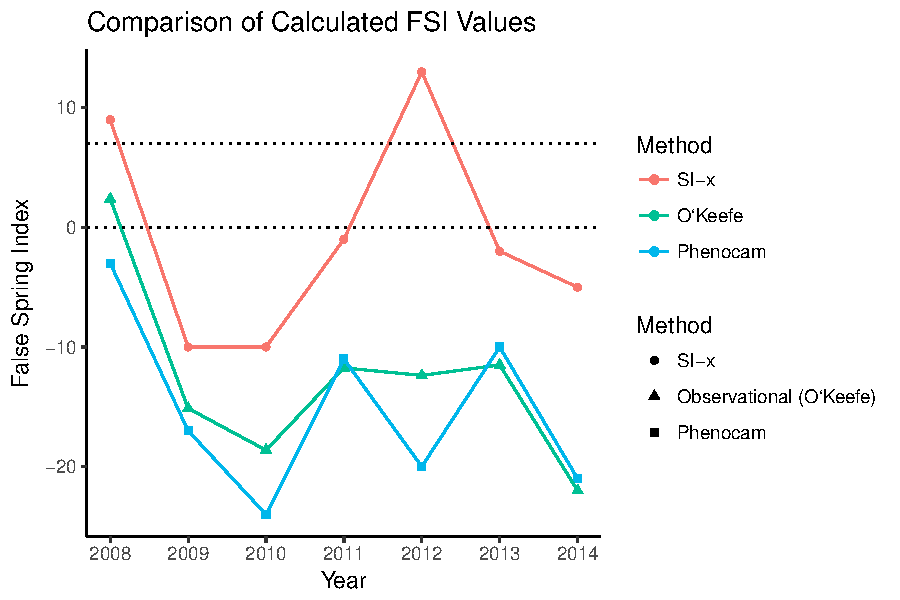
\includegraphics[width=\maxwidth]{figure/fsifig-1} \caption[A scatterplot indicating FSI values from 2008 to 2014 for each methdology used in this study]{A scatterplot indicating FSI values from 2008 to 2014 for each methdology used in this study. PhenoCam FSI values are red, Observed FSI values are blue, and USA-NPN FSI values are green.}\label{fig:fsifig}
\end{figure}



A Pearson Correlation was used to determine the strength of association between the three methods used in the study. As indicated in Table 1, the FSI values from the observed data and the SI-x NPN data are strongly correlated (r=0.93947095), whereas the FSI values calculated using the PhenoCam data is not as strongly correlated to either the observed FSI values (r=0.4679934) or the NPN FSI values (r=0.4242059). Although, according to the pearson correlation, all results were similar. 

\begin{table}[ht]
\centering
\caption{Pearson Correlation Coefficients shown comparing the strength of association between the FSI values calculated across all three methodologies.} 
\begin{tabular}{rrrrr}
  \hline
 & year & npn & okeefe & phenocam \\ 
  \hline
year & 1.00 & -0.03 & -0.20 & -0.37 \\ 
  npn & -0.03 & 1.00 & 0.94 & 0.42 \\ 
  okeefe & -0.20 & 0.94 & 1.00 & 0.47 \\ 
  phenocam & -0.37 & 0.42 & 0.47 & 1.00 \\ 
   \hline
\end{tabular}
\end{table}


Our projections indicate that observational FSI values are highly comparable to the USA-NPN FSI values, rendering both justifiable methods for determining potential risk involved in late spring freezes. Even though budburst is defined differently between Dr. O'Keefe, USA-NPN, and the PhenoCam, the dates of budburst are similar. The spring onset dates gathered from the PhenoCam dataset are different from the other two methods, which is likely due to fact that the PhenoCam data is assessing budburst for the forest canopy. Through the use of USA-NPN data, researchers could gather dates of budburst across multiple locations at once in order to determine False Spring risk, making it a more effective method than observational data. Although, all three methods are viable. It largely depends on the functional group of interest for the study, definition of budburst, and resources available.  

\newpage
\bibliography{..//refs/SpringFreeze.bib}
\end{document}
